%!Tex Program = xelatex
\documentclass{ctexart}
\usepackage{listings}
\usepackage{graphicx}
\usepackage{amsfonts}
\usepackage{float}

\title{作业四:尝试gsl程序的运行}
\author{申屠慧 \\ 能源与环境系统工程(智慧能源班) 3210103417}
\date{\today}
\begin{document}

\maketitle
\section{代码描述}
这段代码是一个使用GNU Scientific Library(GSL)进行样条插值的示例程序。
下面是代码的解释:
\begin{lstlisting}
    #include <stdlib.h>
    #include <stdio.h>
    #include <math.h>
    #include <gsl/gsl_errno.h>
    #include <gsl/gsl_spline.h>
\end{lstlisting}

这些是所需的头文件。
\begin{lstlisting}
    int main (void)
    {
        int i;
        double xi, yi, x[10], y[10];
        printf ("#m=0,S=17\n");
\end{lstlisting}

这里定义了main函数作为程序的入口点,并声明了一些变量。xi和yi是用来存储插值结果的变量,x[10]和y[10]是用来存储插值的数据点的数组。
\begin{lstlisting}
    for (i = 0; i < 10; i++)
    {
        x[i] = i + 0.5 * sin (i);
        y[i] = i + cos (i * i)+3.210103417;
        printf ("%g %g\n", x[i], y[i]);
    }
\end{lstlisting}

这个循环用来填充数据点的数组x和y。其中x[i]通过对i进行sin函数的计算得到,y[i]通过对i进行cos函数的计算得到,并加上一个常数值。

\begin{lstlisting}
    printf ("#m=1,S=0\n");

    {
        gsl_interp_accel *acc = gsl_interp_accel_alloc ();
        gsl_spline *spline = gsl_spline_alloc (gsl_interp_cspline, 10);
        gsl_spline_init (spline, x, y, 10);

\end{lstlisting}

这段代码打印一条注释,并创建了GSL库中的样条插值所需的数据结构。
\begin{lstlisting}
    for (xi = x[0]; xi < x[9]; xi += 0.01)
    {
        yi = gsl_spline_eval (spline, xi, acc);
        printf ("%g %g\n", xi, yi);
    }
\end{lstlisting}

这个循环使用样条插值函数对给定的xi值进行插值,并将结果存储在yi中。然后将xi和yi打印出来。
\begin{lstlisting}
    gsl_spline_free (spline);
    gsl_interp_accel_free (acc);
    }
    return 0;
}
\end{lstlisting}

这段代码释放了之前分配的内存,释放样条插值所需的数据结构。

总体上,这段代码展示了如何使用GSL库进行样条插值。首先生成一组数据点,然后使用样条插值方法对这些数据点进行插值,然后输出插值结果。
\section{代码运行}
\begin{lstlisting}
    gcc -o inter inter.c -lgsl -lm

    ./inter >interp.dat

    graph -T <interp.dat> interp.eps
\end{lstlisting}

\section{生成图片}
\begin{figure}[H]
    \centering
    \includegraphics{interp.eps}
    \caption{生成的图片}
    \label{fig:picture}
\end{figure}

\end{document}